\chapter{Analyse de Sensibilité}
\label{chap:analyse_sensibilite}

Ce chapitre présente une analyse de sensibilité approfondie du modèle étendu pour déterminer l'influence relative des différents paramètres sur les prédictions et quantifier les incertitudes associées.

\section{Méthodologie d'Analyse de Sensibilité}
\label{sec:methodologie_sensibilite}

L'analyse de sensibilité vise à comprendre comment la variabilité des entrées du modèle affecte ses sorties, permettant ainsi d'identifier les paramètres les plus influents et ceux qui pourraient être simplifiés.

\subsection{Approche Globale vs. Locale}
\label{subsec:approche_globale_locale}

Notre analyse combine deux approches complémentaires :

\begin{itemize}
\item \textbf{Analyse de sensibilité locale} : examine l'impact des petites variations d'un paramètre autour de sa valeur de référence, en maintenant les autres paramètres constants.
\item \textbf{Analyse de sensibilité globale} : considère l'espace complet des paramètres et leurs interactions, en échantillonnant dans tout l'espace des paramètres possibles.
\end{itemize}

\subsection{Métriques de Sensibilité}
\label{subsec:metriques_sensibilite}

Plusieurs métriques sont utilisées pour quantifier la sensibilité :

\begin{itemize}
\item \textbf{Coefficients de sensibilité normalisés} pour l'analyse locale :
\begin{equation}
S_i = \frac{\partial y}{\partial \theta_i} \cdot \frac{\theta_i}{y}
\end{equation}
où $y$ est la sortie du modèle et $\theta_i$ le paramètre étudié.

\item \textbf{Indices de Sobol'} pour l'analyse globale, mesurant la contribution de chaque paramètre à la variance totale de la sortie :
\begin{equation}
S_i = \frac{\text{Var}_{\theta_i}(E_{\theta_{\sim i}}[y|\theta_i])}{\text{Var}(y)}
\end{equation}
où $\theta_{\sim i}$ représente tous les paramètres sauf $\theta_i$.

\item \textbf{Distance de Wasserstein} entre les distributions de sortie, pour évaluer l'impact des variations de paramètres sur l'ensemble de la distribution :
\begin{equation}
W_p(F_1, F_2) = \left( \inf_{\gamma \in \Gamma(F_1, F_2)} \int_{X \times X} d(x, y)^p d\gamma(x, y) \right)^{1/p}
\end{equation}
où $F_1$ et $F_2$ sont deux distributions, et $\Gamma(F_1, F_2)$ l'ensemble des distributions jointes possibles.
\end{itemize}

\section{Étude Quantitative des Paramètres}
\label{sec:etude_quantitative}

Nous appliquons ces méthodes pour analyser la sensibilité du modèle aux différents paramètres, en nous concentrant sur leurs effets sur les variables macroscopiques du trafic.

\subsection{Sensibilité aux Paramètres des Fonctions de Modulation}
\label{subsec:sensibilite_modulation}

L'analyse de l'influence des paramètres $\etaM$ (coefficient de gap-filling) et $\mui{i}$ (coefficients d'interweaving) révèle :

\begin{figure}[htbp]
\centering
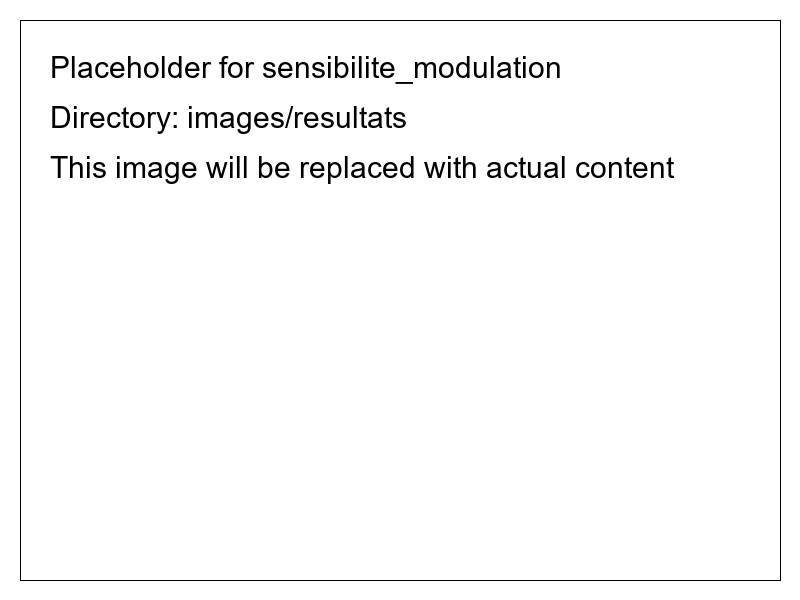
\includegraphics[width=0.9\textwidth]{images/resultats/sensibilite_modulation}
\caption{Analyse de sensibilité aux paramètres des fonctions de modulation : (a) influence de $\etaM$ sur la vitesse des motos; (b) influence de $\mui{i}$ sur les autres classes; (c) indices de Sobol' pour ces paramètres.}
\label{fig:sensibilite_modulation}
\end{figure}

\begin{itemize}
\item Le coefficient $\etaM$ a un impact modéré sur la vitesse des motos ($S_{\etaM} = 0.31$), avec une influence croissante à mesure que la densité des motos augmente.
\item Les coefficients $\mui{i}$ ont une influence variable selon la classe de véhicule, avec un impact particulièrement important pour les bus et camions ($S_{\mu_{\text{bus}}} = 0.57$, $S_{\mu_{\text{camion}}} = 0.62$).
\item L'indice de Sobol' de second ordre $S_{\etaM,\mui{i}}$ montre une interaction significative entre ces paramètres, indiquant que leurs effets ne sont pas simplement additifs.
\end{itemize}

\subsection{Sensibilité au Coefficient de Ralentissement}
\label{subsec:sensibilite_ralentissement}

Le coefficient de ralentissement lié au revêtement $\matcoef{i}$ joue un rôle crucial dans la dynamique du modèle :

\begin{figure}[htbp]
\centering
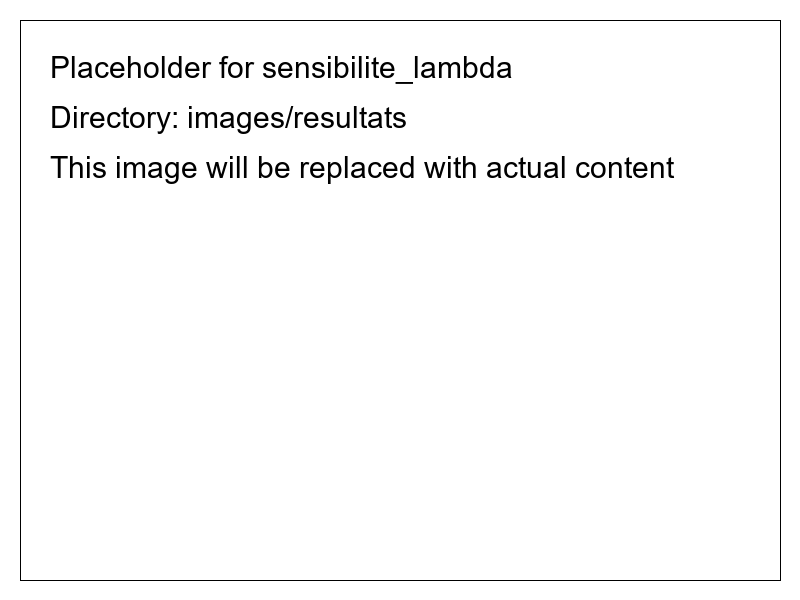
\includegraphics[width=0.9\textwidth]{images/resultats/sensibilite_lambda}
\caption{Sensibilité au coefficient de ralentissement $\matcoef{i}$ : (a) impact sur la vitesse moyenne; (b) impact sur le flux; (c) propagation de l'incertitude dans le modèle.}
\label{fig:sensibilite_lambda}
\end{figure}

L'analyse révèle :
\begin{itemize}
\item Une relation quasiment linéaire entre $\matcoef{i}$ et la vitesse moyenne pour toutes les classes de véhicules ($S_{\matcoef{i}} \approx 1$).
\item Un impact non-linéaire sur le flux, particulièrement prononcé dans les régimes de densité intermédiaire.
\item Une sensibilité différenciée selon les classes de véhicules, les motos étant moins sensibles aux variations de $\matcoef{i}$ que les autres classes.
\end{itemize}

\subsection{Sensibilité aux Paramètres Fondamentaux}
\label{subsec:sensibilite_fondamentaux}

Les paramètres fondamentaux du modèle LWR étendu incluent la vitesse libre de référence $\maxveli{i}$ et la densité maximale $\maxdens_i$ :

\begin{table}[htbp]
\centering
\caption{Indices de sensibilité pour les paramètres fondamentaux}
\label{tab:indices_sensibilite}
\begin{tabular}{lcc}
\toprule
\textbf{Paramètre} & \textbf{Indice de Sobol' (1er ordre)} & \textbf{Indice total} \\
\midrule
$v_{M,\max}^0$ (vitesse libre des motos) & 0.48 & 0.56 \\
$v_{\text{voiture},\max}^0$ (vitesse libre des voitures) & 0.35 & 0.41 \\
$\rho_{M,\max}$ (densité max des motos) & 0.38 & 0.44 \\
$\rho_{\text{voiture},\max}$ (densité max des voitures) & 0.22 & 0.29 \\
\bottomrule
\end{tabular}
\end{table}

Ces résultats montrent :
\begin{itemize}
\item Une influence prédominante des paramètres liés aux motos, confirmant leur rôle central dans la dynamique du trafic béninois.
\item Des interactions modérées entre les paramètres (différence entre indices totaux et de premier ordre), suggérant des effets synergiques.
\end{itemize}

\section{Simulations Monte Carlo}
\label{sec:monte_carlo}

Pour quantifier l'incertitude globale du modèle et sa propagation, des simulations de Monte Carlo ont été réalisées.

\subsection{Méthodologie des Simulations}
\label{subsec:methodologie_monte_carlo}

La procédure suivie comprend les étapes suivantes :

\begin{enumerate}
\item Définition des distributions de probabilité pour chaque paramètre, basées sur les intervalles de confiance de la calibration.
\item Génération de $N=1000$ jeux de paramètres par échantillonnage latin hypercube (LHS).
\item Exécution du modèle pour chaque jeu de paramètres.
\item Analyse statistique des résultats : distributions de probabilité des sorties, intervalles de confiance, etc.
\end{enumerate}

\subsection{Propagation des Incertitudes}
\label{subsec:propagation}

L'analyse de la propagation des incertitudes à travers le modèle montre comment les incertitudes sur les paramètres se traduisent par des incertitudes sur les prédictions :

\begin{figure}[htbp]
\centering
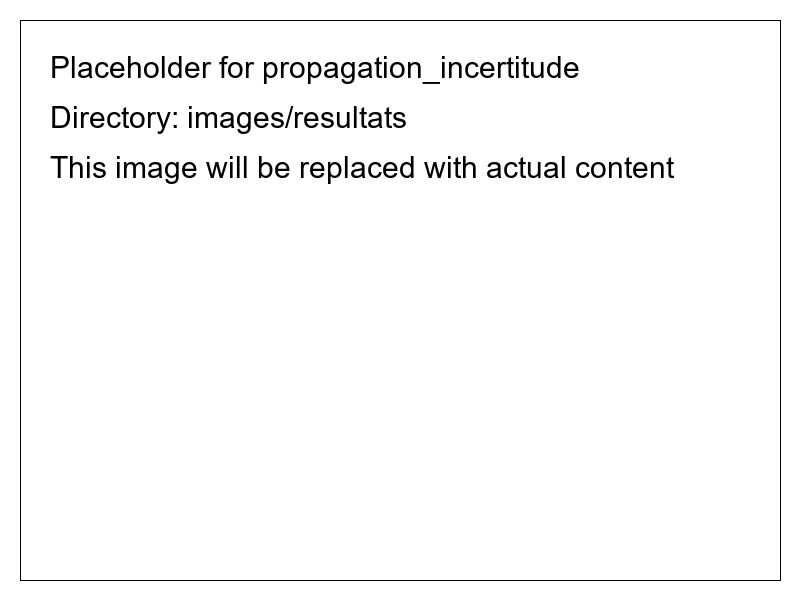
\includegraphics[width=0.9\textwidth]{images/resultats/propagation_incertitude}
\caption{Propagation des incertitudes : (a) distribution des vitesses prédites; (b) distribution des flux prédits; (c) incertitude en fonction de la densité.}
\label{fig:propagation_incertitude}
\end{figure}

Observations principales :
\begin{itemize}
\item L'incertitude relative sur le flux (mesurée par le coefficient de variation) est plus importante dans les régimes de densité intermédiaire (proche de la densité critique).
\item Les prédictions concernant les motos présentent une incertitude plus faible que celles des autres classes, reflétant la plus grande robustesse de cette classe aux variations de paramètres.
\item L'incertitude augmente significativement lorsque plusieurs types de véhicules interagissent fortement, notamment aux densités élevées.
\end{itemize}

\subsection{Analyse des Scénarios Extrêmes}
\label{subsec:scenarios_extremes}

L'analyse des scénarios correspondant aux quantiles extrêmes (5\% et 95\%) des distributions de sortie permet d'évaluer la robustesse du modèle face à des combinaisons défavorables de paramètres :

\begin{table}[htbp]
\centering
\caption{Analyse des scénarios extrêmes}
\label{tab:scenarios_extremes}
\begin{tabular}{lccc}
\toprule
\textbf{Variable} & \textbf{Quantile 5\%} & \textbf{Valeur médiane} & \textbf{Quantile 95\%} \\
\midrule
Vitesse moyenne des motos (km/h) & 42.3 & 48.5 & 53.8 \\
Vitesse moyenne des voitures (km/h) & 35.6 & 42.9 & 49.2 \\
Flux total maximal (véh/h) & 8320 & 9450 & 10620 \\
Densité critique (véh/km) & 75.8 & 86.3 & 97.1 \\
\bottomrule
\end{tabular}
\end{table}

Ces résultats montrent une plage d'incertitude acceptable pour les applications pratiques du modèle, avec une variation de l'ordre de $\pm$15\% autour de la valeur médiane pour les principales variables de trafic.

\section{Classification des Paramètres par Importance}
\label{sec:classification_parametres}

En synthétisant les résultats des analyses de sensibilité locale et globale, nous pouvons classifier les paramètres par ordre d'importance :

\begin{figure}[htbp]
\centering
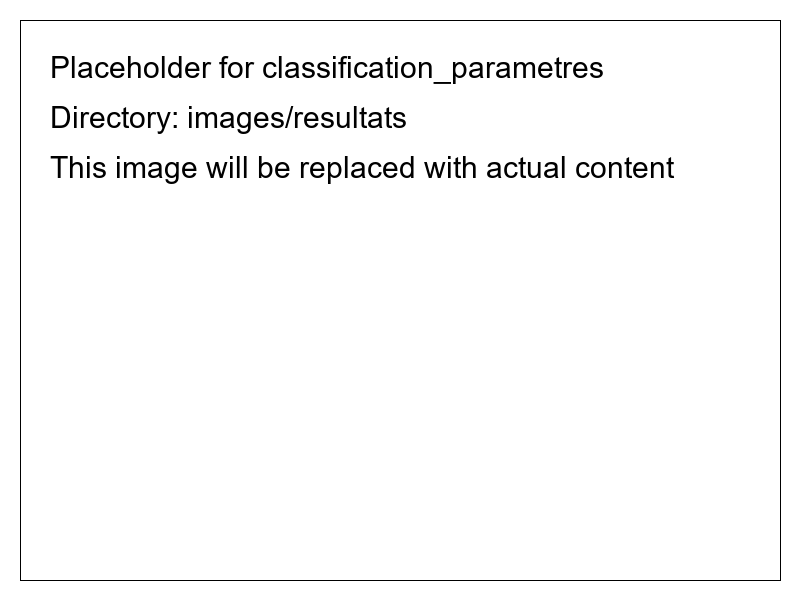
\includegraphics[width=0.8\textwidth]{images/resultats/classification_parametres}
\caption{Classification des paramètres du modèle selon leur importance relative.}
\label{fig:classification_parametres}
\end{figure}

Cette classification révèle trois groupes de paramètres :

\begin{enumerate}
\item \textbf{Paramètres critiques} (forte influence) : 
   \begin{itemize}
   \item Vitesse libre de référence des motos $v_{M,\max}^0$
   \item Coefficient de ralentissement des voitures $\lambda_{\text{mat,voiture}}$
   \item Coefficient d'interweaving pour les camions $\mu_{\text{camion}}$
   \end{itemize}

\item \textbf{Paramètres importants} (influence modérée) : 
   \begin{itemize}
   \item Densité maximale des motos $\rho_{M,\max}$
   \
